% \ がすべて ¥ になっていたので修正
\documentclass[./main]{subfiles}

\begin{document}

\Chapter{パズルのコーナー(まどれ〜ぬ)} 
\Section{ピラミッド}
\noindent 〈ルール〉1.全てのマスに1〜9の数字のうちどれかひとつを書き込みます。\\
 2.同じ高さの段で、同じ数字が2つ以上入ることはありません。\\
 3.一番下の段を除く全てのマスで、そこに入る数字はそのマスの下にある数字の和か差になります。\\
 4.点線で囲まれた枠では、中に入る数字の合計が、左上に書かれた数字と同じになります。\\[15pt]
                例題              例題の答え
\begin{center}
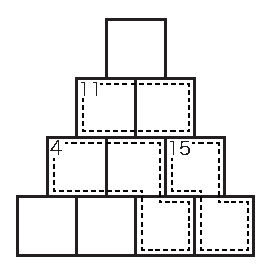
\includegraphics{manuscript/morikawa_image/morikawa_puzzle_inst_p.eps}     
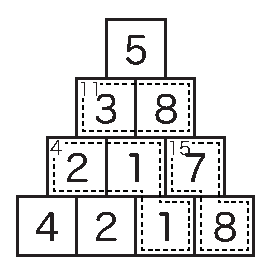
\includegraphics{manuscript/morikawa_image/morikawa_puzzle_inst_a.eps}
\end{center}
\begin{minipage}{0.4375\hsize}
\vspace{15pt}1.\vspace{-15pt}
\begin{center}
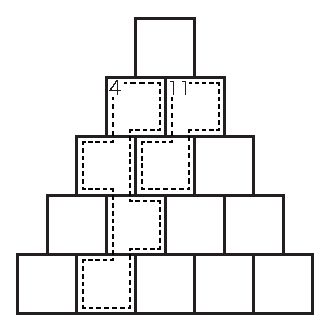
\includegraphics{manuscript/morikawa_image/morikawa_puzzle_1.eps}
\end{center}
\vspace{15pt}2.\vspace{-15pt}
\begin{center}
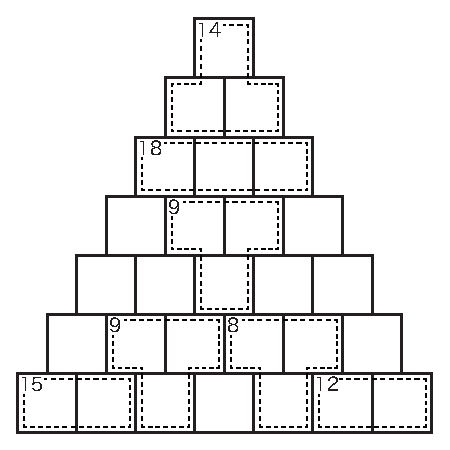
\includegraphics{manuscript/morikawa_image/morikawa_puzzle_2.eps}
\end{center}
\end{minipage}
\begin{minipage}{0.5625\hsize}
\vspace{15pt}3.\vspace{-15pt}
\begin{center}
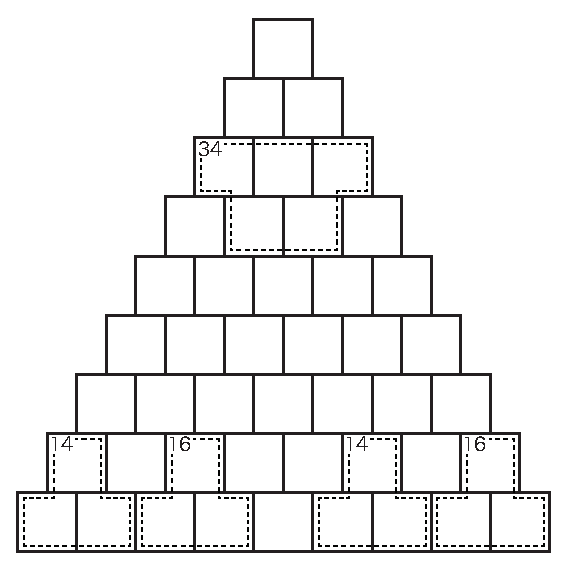
\includegraphics{manuscript/morikawa_image/morikawa_puzzle_3.eps}
\end{center}
\end{minipage}
\end{document}

%¥begin{thebibliography}{9}
%¥item Hull, J. C. (2014), Options, Futures, and Other Derivatives, 9th edition (Upper Saddle River, NJ: Prentice Hall).
%¥end{thebibliography}
